% Constitutional Hash: cdd01ef066bc6cf2
\section{Discussion}\label{sec:discussion}

Our prototype development and controlled testing reveal a fundamental challenge for constitutional AI research: the \textbf{synthetic constitution problem}. Laboratory validation with researcher-designed constitutions provides limited insight into system behavior under authentic governance conditions. This discussion confronts this limitation directly, analyzing the laboratory-to-production gap, the deliberation-performance tension, and critical boundary conditions that define appropriate application scope for constitutional AI infrastructure.

\subsection{The Constitutional Infrastructure Paradigm}

Our synthetic scenario analysis supports positioning ACGS-2 as
\textbf{constitutional infrastructure} rather than constitutional automation.
The system's design prioritizes enabling democratic processes while preserving
human authority over constitutional interpretation. Validation with authentic
stakeholders remains essential to confirm the effectiveness of this positioning.

\subsubsection{Design Principles for Infrastructure Effectiveness}

Three design principles support the infrastructure paradigm:

\paragraph{Deliberative Process Preservation.} Despite sub-millisecond automated reasoning capabilities, the system architecture
is designed to maintain meaningful stakeholder consultation periods (governance
literature suggests days to weeks are typical), demonstrating that technical
efficiency can potentially coexist with democratic deliberation when systems are
designed as enablers rather than replacements.

\paragraph{Stakeholder Agency Mechanisms.} The system includes appeal processes and consultation integration mechanisms
designed to ensure stakeholders retain meaningful influence over constitutional
decisions. Synthetic scenario testing validates these mechanisms function
correctly, though validation with authentic stakeholders is needed to confirm
they adequately support democratic participation.

\paragraph{Constitutional Evolution Support.} The system architecture supports constitutional amendment processes,
enabling constitutional change through democratic mechanisms rather than purely
technical optimization. The effectiveness of these features requires validation
through longitudinal studies with real governance communities.

\subsubsection{The Deliberation-Performance Tension}

A fundamental tension exists between technical performance optimization and democratic legitimacy: systems optimized for millisecond response times operate at timescales fundamentally incompatible with meaningful human deliberation. Figure~\ref{fig:temporal_mismatch} illustrates this \textbf{temporal mismatch}---constitutional reasoning operates at millisecond scales while democratic deliberation requires days to years. Our design attempts to manage this tension by positioning technical speed as infrastructure enabler rather than deliberation replacement:

\begin{itemize}[itemsep=2pt,parsep=1pt]
    \item \textbf{Technical Speed as Enabler}: Sub-millisecond reasoning enables rapid constitutional consistency checking designed to support rather than replace human deliberation
    \item \textbf{Efficiency for Infrastructure}: Sustained throughput meeting targets in controlled tests (\throughputrange) provides the foundation for reliable infrastructure, though real-world democratic process integration requires validation
    \item \textbf{Transparency as Design Priority}: The system prioritizes decision transparency and explainable automated reasoning to build trust rather than undermine democratic oversight, though effectiveness requires validation with authentic stakeholders
\end{itemize}

\begin{figure}[htbp]
\centering
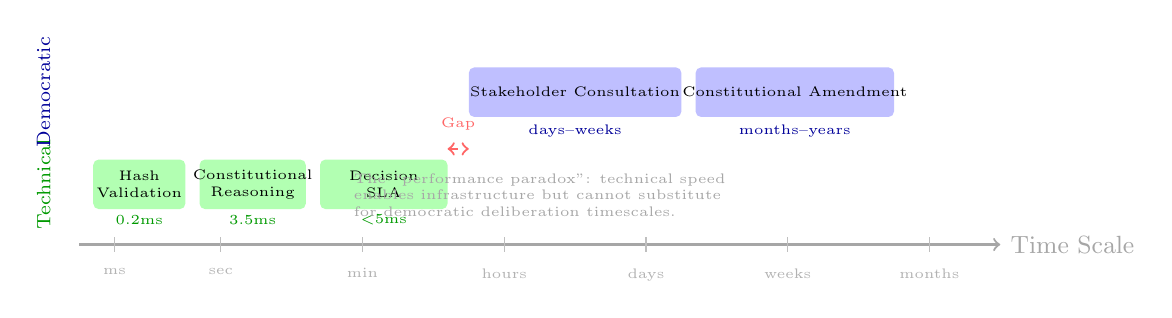
\begin{tikzpicture}[scale=0.9]
    % Time axis (logarithmic scale representation)
    \draw[->, thick, gray!70] (0,0) -- (13,0) node[right, font=\small] {Time Scale};

    % Time scale labels
    \foreach \x/\lab in {0.5/ms, 2/sec, 4/min, 6/hours, 8/days, 10/weeks, 12/months} {
        \draw[gray!50] (\x,-0.1) -- (\x,0.1);
        \node[below, font=\tiny, gray!60] at (\x,-0.2) {\lab};
    }

    % Technical processes (bottom, green)
    \fill[green!30, rounded corners=2pt] (0.2,0.5) rectangle (1.5,1.2);
    \node[font=\tiny, align=center] at (0.85,0.85) {Hash\\Validation};
    \node[font=\tiny, green!60!black] at (0.85,0.35) {0.2ms};

    \fill[green!30, rounded corners=2pt] (1.7,0.5) rectangle (3.2,1.2);
    \node[font=\tiny, align=center] at (2.45,0.85) {Constitutional\\Reasoning};
    \node[font=\tiny, green!60!black] at (2.45,0.35) {3.5ms};

    \fill[green!30, rounded corners=2pt] (3.4,0.5) rectangle (5.2,1.2);
    \node[font=\tiny, align=center] at (4.3,0.85) {Decision\\SLA};
    \node[font=\tiny, green!60!black] at (4.3,0.35) {<5ms};

    % Democratic processes (top, blue)
    \fill[blue!25, rounded corners=2pt] (5.5,1.8) rectangle (8.5,2.5);
    \node[font=\tiny, align=center] at (7,2.15) {Stakeholder Consultation};
    \node[font=\tiny, blue!60!black] at (7,1.6) {days--weeks};

    \fill[blue!25, rounded corners=2pt] (8.7,1.8) rectangle (11.5,2.5);
    \node[font=\tiny, align=center] at (10.1,2.15) {Constitutional Amendment};
    \node[font=\tiny, blue!60!black] at (10.1,1.6) {months--years};

    % Gap annotation
    \draw[<->, red!60, thick, dashed] (5.2,1.35) -- (5.5,1.35);
    \node[font=\tiny, red!60, align=center] at (5.35,1.7) {Gap};

    % Labels
    \node[font=\scriptsize, green!60!black, rotate=90] at (-0.5,0.85) {Technical};
    \node[font=\scriptsize, blue!60!black, rotate=90] at (-0.5,2.15) {Democratic};

    % Legend annotation
    \node[font=\tiny, align=left, gray!70] at (6.5,0.7) {The ``performance paradox'': technical speed\\enables infrastructure but cannot substitute\\for democratic deliberation timescales.};
\end{tikzpicture}
\caption{Temporal mismatch between technical automation and democratic deliberation. Green boxes show technical process timescales (milliseconds); blue boxes show democratic governance timescales (days to years). The fundamental tension: constitutional AI can enable rapid consistency checking but cannot compress the deliberation time essential for democratic legitimacy.}
\label{fig:temporal_mismatch}
\Description{Timeline diagram showing temporal scales from milliseconds to months. Technical processes (hash validation 0.2ms, constitutional reasoning 3.5ms, decision SLA <5ms) shown in green on the left. Democratic processes (stakeholder consultation days--weeks, constitutional amendment months--years) shown in blue on the right. A gap between the two clusters highlights the fundamental temporal mismatch that constitutional AI systems must navigate.}
\end{figure}

\subsection{The Laboratory-to-Production Gap}

The gap between controlled testing and production deployment represents a critical uncertainty in constitutional AI research. Our laboratory metrics (\pnnlatency{} P99 latency, \throughput{} throughput, \constitutionalcompliance{} compliance) reflect idealized conditions: synthetic workloads, deterministic networks, and researcher-designed constitutions. Production deployment would introduce network variability, authentic stakeholder conflicts, and constitutional complexity that cannot be captured in laboratory settings.

\subsubsection{Implications for Claims and Generalization}

This gap has three implications that constrain how laboratory results should be interpreted:

\paragraph{Ecological Validity Considerations.} Laboratory validation with synthetic constitutional frameworks provides limited
predictive value for production performance. Real constitutional complexity,
stakeholder conflicts, and governance ambiguity would likely challenge automated
reasoning systems in ways that synthetic scenarios cannot fully capture.

\paragraph{Stakeholder Integration Requirements.} Based on governance literature, meaningful democratic participation requires
substantial deliberation time (typically days to weeks) that cannot be optimized
away without sacrificing legitimacy. This supports our theoretical framework
positioning deliberation time as essential rather than inefficient.

\paragraph{Infrastructure vs. Automation Trade-offs.} The infrastructure approach prioritizes democratic process support over
pure performance optimization, which may prove more robust to real-world
deployment challenges than automation approaches that optimize primarily for
laboratory benchmarks.

\subsubsection{Expected Deployment Considerations}

Based on our development experience and distributed systems literature,
organizations considering constitutional AI deployment should anticipate:
\begin{itemize}[itemsep=1pt,parsep=1pt]
    \item \textbf{Performance Variation}: Estimated 2--4x impact from infrastructure variability and stakeholder integration
    \item \textbf{Stakeholder Integration Time}: Days to weeks for meaningful consultation processes (based on governance literature)
    \item \textbf{Infrastructure Investment}: Substantial technical expertise required for production deployment
    \item \textbf{Ongoing Democratic Maintenance}: Constitutional frameworks would require continuous stakeholder engagement for legitimacy preservation
\end{itemize}

\subsection{The Synthetic Constitution Problem}

The \textbf{synthetic constitution problem} represents a central methodological challenge for constitutional AI research: systems validated against researcher-designed frameworks may perform very differently against authentic constitutions developed through democratic processes. This problem manifests through three interconnected mechanisms that define limits of laboratory validation:

\subsubsection{Ambiguity Resolution Challenges}

Laboratory constitutional frameworks necessarily eliminate ambiguity for
computational tractability. Production frameworks would maintain intentional
ambiguity for contextual interpretation, creating an anticipated
\textbf{ambiguity gap} for authentic constitutional governance.

Our synthetic scenario analysis reveals systematic challenges around ambiguous
constitutional interpretation scenarios, suggesting that ambiguity handling
represents a key area where synthetic validation cannot fully predict real-world
performance.

\subsubsection{Anticipated Stakeholder Conflict Challenges}

Synthetic frameworks avoid stakeholder conflicts for validation consistency.
Real-world deployments would need to navigate authentic conflicts between
competing stakeholder groups across domains:
\begin{itemize}[itemsep=1pt,parsep=1pt]
    \item Healthcare: Patient privacy advocates vs. medical transparency requirements
    \item Finance: Consumer protection advocates vs. financial institution risk management
    \item Education: Student privacy advocates vs. parental rights
    \item Government: Transparency advocates vs. security requirements
\end{itemize}

The system includes conflict resolution mechanisms, but their effectiveness for
authentic stakeholder conflicts requires validation with real governance
communities.

\subsubsection{Constitutional Evolution Considerations}

Synthetic constitutions remain static for validation repeatability. Authentic
constitutions evolve through democratic processes, creating ongoing adaptation
challenges. Based on governance literature:
\begin{itemize}[itemsep=1pt,parsep=1pt]
    \item Constitutional amendment processes typically span months to years
    \item Technical systems must adapt to democratically-approved changes
    \item Continuous stakeholder engagement is essential for legitimacy
\end{itemize}

The system architecture supports constitutional evolution, but long-term
effectiveness requires longitudinal studies with authentic governance
communities.

\subsection{Critical Limitations and Boundary Conditions}

Honest assessment of ACGS-2's limitations is essential for responsible positioning of this research. We identify three categories of constraints: technical architecture limitations that bound system capabilities, democratic legitimacy constraints that frame the fundamental role of human authority, and societal implications that require ongoing attention.

\subsubsection{Technical Architecture Limitations}

\paragraph{Engineering Integration vs. Algorithmic Innovation.} ACGS-2 represents sophisticated engineering integration of established
techniques rather than fundamental algorithmic contributions. The
constitutional hash mechanism applies standard cryptographic methods,
multi-tier validation combines existing tools (OPA/Rego, Transformer models, Z3
SMT solver), and microservices architecture follows established distributed
systems patterns.

Our contribution is demonstrating that these techniques can be successfully
integrated for constitutional governance prototypes, but the underlying
technical methods are incremental rather than novel.

\paragraph{Scalability Considerations.} Based on our controlled testing, we identify scalability considerations:
\begin{itemize}[itemsep=1pt,parsep=1pt]
    \item Constitutional complexity likely increases sublinearly with stakeholder count,
          potentially limiting scalability for large democratic communities
    \item Transformer-based reasoning has memory requirements that may constrain
          concurrent decision capacity at scale
    \item Stakeholder integration overhead would grow with democratic participation
          requirements
    \item Cross-jurisdictional constitutional coordination remains entirely unvalidated
\end{itemize}

\paragraph{Constitutional Reasoning Depth Limitations.} Multi-modal reasoning capabilities, while functional in synthetic scenarios,
have inherent limitations. Based on our analysis, we anticipate systematic gaps
in production deployment:
\begin{itemize}[itemsep=1pt,parsep=1pt]
    \item Cultural context integration: Synthetic scenarios cannot capture cultural
          nuances in constitutional interpretation
    \item Historical precedent application: System has limited ability to incorporate
          evolving constitutional precedent
    \item Cross-jurisdictional principle synthesis: Not validated for
          multi-jurisdictional constitutional coordination
    \item Moral reasoning under uncertainty: Automated systems have fundamental
          limitations in ethical reasoning requiring human judgment
\end{itemize}

\subsubsection{Democratic Legitimacy Constraints}

\paragraph{Constitutional Design Authority.} ACGS-2 provides infrastructure for constitutional enforcement but does not
address fundamental questions of constitutional design authority. Who has
legitimacy to design initial constitutional frameworks? How are constitutional
amendments democratically authorized? How is stakeholder representation equity
maintained over time?

Our technical infrastructure supports but cannot resolve these inherently
political questions. Constitutional amendment support mechanisms are included
in the system architecture, but their effectiveness in supporting authentic
constitutional evolution requires validation with real governance communities.

\paragraph{Power Concentration Risks.} Technical systems for constitutional governance may concentrate power in ways
that undermine democratic distribution of authority. Six specific risks
require ongoing attention:
\begin{enumerate}[itemsep=1pt,parsep=1pt]
    \item \textbf{Constitutional Capture}: Well-resourced actors may disproportionately influence initial constitutional design, embedding favorable principles before democratic processes can meaningfully engage~\cite{delacroix2023algorithmic}
    \item \textbf{Algorithmic Lock-in}: Once constitutional frameworks are technically encoded, path dependencies may make democratic revision prohibitively difficult, ossifying governance arrangements that would otherwise evolve through deliberation
    \item \textbf{Epistemic Injustice}: Communities whose governance traditions rely on oral histories, contextual wisdom, or non-Western deliberative practices may find their constitutional contributions systematically undervalued by systems requiring formal specification~\cite{Habermas1996BetweenFacts}
    \item \textbf{Technical Capture}: Constitutional frameworks designed by technical teams may embed particular political or cultural assumptions
    \item \textbf{Elite Participation Bias}: Sophisticated technical systems may favor stakeholders with technical expertise or resources
    \item \textbf{Process Formalization Bias}: Technical requirements for formal constitutional specification may favor explicit rules over cultural norms and contextual wisdom
\end{enumerate}

\paragraph{Algorithmic Discretion and Mercy.} Constitutional governance often requires discretion, mercy, and contextual
exceptions that resist formal specification. High compliance rates with formal
rules, while technically desirable, may represent a level of rigidity that is
inappropriate for complex moral and social situations requiring human judgment
and contextual interpretation.

This represents a fundamental limitation of automated constitutional
enforcement: formal systems cannot fully capture the nuance of human judgment
in cases requiring exceptions based on extraordinary circumstances,
compassionate considerations, or evolving community values.

\subsubsection{Societal and Ethical Implications}

\paragraph{Digital Governance Inequality.} Constitutional AI systems with ACGS-2's complexity would require substantial
resource investment (significant operational costs and specialized engineering
teams), potentially limiting accessibility to well-funded organizations. This
resource requirement risks exacerbating digital governance inequality rather
than democratizing access to constitutional AI infrastructure.

Smaller organizations and communities requiring constitutional governance may
lack resources for sophisticated technical implementation, potentially creating
two-tier governance systems where technical sophistication correlates with
democratic infrastructure quality. Research on simplified, community-accessible
constitutional AI infrastructure remains essential.

\paragraph{Governance Failure Mode Ethics.} Constitutional AI systems can fail in multiple ways with distinct ethical
implications:
\begin{itemize}[itemsep=1pt,parsep=1pt]
    \item \textbf{Failing Closed}: Denying legitimate constitutional rights when systems are unavailable
    \item \textbf{Failing Open}: Allowing constitutionally prohibited actions when governance systems are compromised
    \item \textbf{Failing Partially}: Inconsistent constitutional enforcement creating fairness issues across different system components
\end{itemize}

Our technical architecture includes circuit breakers and graceful degradation,
but the ethical framework for determining appropriate failure behaviors remains
an open challenge requiring ongoing democratic deliberation.

\paragraph{Connection to AI Safety Research.} ACGS-2 addresses several ``concrete problems in AI safety''~\cite{Amodei2016ConcreteProblems} through constitutional mechanisms: safe interruptibility through appeal processes, avoiding negative side effects via multi-stakeholder constitutional constraints, and scalable oversight through formal verification. However, our synthetic validation cannot assess whether these safety properties transfer to deployment with authentic constitutional frameworks. As Russell~\cite{Russell2019HumanCompatible} argues, AI systems must remain fundamentally uncertain about human preferences; constitutional AI infrastructure should similarly remain humble about encoding constitutional principles that may require ongoing democratic refinement.

\subsection{Future Research Directions}

Our prototype development and synthetic validation generate several critical
research directions for advancing constitutional AI as democratic
infrastructure.

\subsubsection{Constitutional Legitimacy and Democratic Design}

\paragraph{Participatory Constitutional Design Methods.} How can technical systems support authentic participatory processes for
constitutional design and evolution? Our development experience suggests this
requires methods for:
\begin{itemize}[itemsep=1pt,parsep=1pt]
    \item Large-scale stakeholder engagement with meaningful participation (beyond
          consultation)
    \item Cultural context integration that preserves community values and norms
    \item Constitutional amendment processes that balance stability with democratic
          evolution
    \item Cross-community constitutional coordination without homogenization
\end{itemize}

\paragraph{Democratic Legitimacy Metrics.} How should constitutional AI systems measure and optimize for democratic
legitimacy rather than technical performance? Our DFC metric provides a
starting point, but further research is needed on:
\begin{itemize}[itemsep=1pt,parsep=1pt]
    \item Stakeholder representation equity measurement and maintenance
    \item Democratic participation quality assessment beyond satisfaction surveys
    \item Constitutional evolution indicators that distinguish healthy adaptation from
          illegitimate drift
    \item Cross-cultural democratic legitimacy criteria that respect diverse governance
          traditions
\end{itemize}

\subsubsection{Technical Architecture Research}

\paragraph{Human-AI Constitutional Collaboration.} How can constitutional AI systems be designed to enhance rather than replace
human constitutional reasoning? Priority research areas include:
\begin{itemize}[itemsep=1pt,parsep=1pt]
    \item Constitutional reasoning explanation that enables meaningful human oversight
    \item Human constitutional wisdom integration into automated decision-making
    \item Constitutional exception and discretion mechanisms that preserve human judgment
    \item Collaborative constitutional interpretation that combines human insight with
          technical consistency
\end{itemize}

\paragraph{Cross-Jurisdictional Constitutional Coordination.} How can constitutional AI systems support governance across multiple legal and
cultural jurisdictions? Our single-jurisdiction validation leaves this largely
unexplored:
\begin{itemize}[itemsep=1pt,parsep=1pt]
    \item Constitutional principle translation across legal traditions and cultural
          contexts
    \item Multi-jurisdictional conflict resolution for competing constitutional
          requirements
    \item Federal/subsidiary constitutional coordination with preserved local autonomy
    \item International constitutional cooperation mechanisms for global governance
          challenges
\end{itemize}

\subsubsection{Sociotechnical Governance Research}

\paragraph{Constitutional AI Ethics and Power Distribution.} How can constitutional AI systems be designed and deployed to distribute rather
than concentrate democratic power? Research priorities include:
\begin{itemize}[itemsep=1pt,parsep=1pt]
    \item Democratic control mechanisms for constitutional AI system governance
    \item Power distribution analysis and equity measurement in technical governance
          systems
    \item Constitutional AI accessibility and digital governance inequality mitigation
    \item Community sovereignty preservation in technical constitutional implementation
\end{itemize}

\paragraph{Long-term Constitutional Evolution.} How do constitutional AI systems affect constitutional evolution and democratic
adaptation over time? Longitudinal studies are needed on:
\begin{itemize}[itemsep=1pt,parsep=1pt]
    \item Constitutional calcification risks from technical enforcement
    \item Democratic learning and constitutional wisdom accumulation over time
    \item Constitutional system resilience to social, technological, and political change
    \item Intergenerational constitutional justice and evolving community values
\end{itemize}

\subsection{Implications for the FAccT Community}

This work contributes to the FAccT community's interdisciplinary mission by
exploring both the potential and limitations of technical approaches to
fairness, accountability, and transparency in governance systems.

\subsubsection{Methodological Contributions}

Our research methodology establishes precedent for evaluating fairness,
accountability, and transparency systems based on their capacity to support
rather than replace human judgment and democratic deliberation. The proposed
Democratic Facilitation Capacity metric provides a template for assessing
sociotechnical systems beyond technical performance optimization, though it
requires empirical validation with authentic stakeholders.

\subsubsection{Critical Technical Analysis}

By providing honest analysis of both technical capabilities and fundamental
limitations---including explicit acknowledgment of synthetic data
constraints---this work models the kind of critical technical analysis
essential for responsible AI development. The laboratory-to-production gap
analysis demonstrates the importance of ecological validity in fairness and
accountability research.

\subsubsection{Democratic Technology Design}

ACGS-2's positioning as constitutional infrastructure rather than
constitutional automation provides a framework for designing technical systems
that aim to enhance democratic processes rather than bypass them. This approach
may inform broader discussions about the appropriate scope of automation in
socially consequential decision-making.

Our prototype development suggests that technical systems can potentially
support fairness, accountability, and transparency in governance contexts when
designed as infrastructure for human decision-making rather than as
replacements for human judgment. Validation with authentic stakeholders is
required to confirm this potential. This framework may prove applicable beyond
constitutional governance to other domains where automated decision-making
intersects with democratic values and social justice concerns.
